% Drawing 122/01-1 -- folder 122, batch 01, archive page 2 (PDF page 3).
% Transcription: en bas à gauche, un croquis : un anneau hachuré $\widetilde{\partial P}$ bordé par le cercle $\partial P$
% Kind: hatched annulus bordered by a circle. Method 2 (schematic redraw from the facsimile). Status: ok.
% Notes: An annulus between two circles, hatched by short radial strokes (their number schematised), labelled with the tilde-boundary of P inside at the top; the outer circle is labelled del P at the right.
% Coordinates: 1 unit = 1 mm = 1/100 of the crop width (bbox in page fractions: [0.06, 0.76, 0.24, 0.88]).
% Redrawn by Claude (claude-opus-5-5), issue #73, 2026-11-07; not checked by a human; not compiled (no TeX in the session).
% Rights: reproduces part of the work -- behind RENDER_TRANSCRIPTS, never published by itself.
\documentclass[tikz,border=3pt]{standalone}
\usepackage{amsmath,amssymb}
\usetikzlibrary{patterns,arrows.meta}
\tikzset{pencil/.style={black!45}, struck/.style={black!35}, mark/.style={circle,draw,inner sep=1.3pt}, pt/.style={circle,fill,inner sep=0.9pt}, opt/.style={circle,draw,fill=white,inner sep=1.1pt}}
\begin{document}
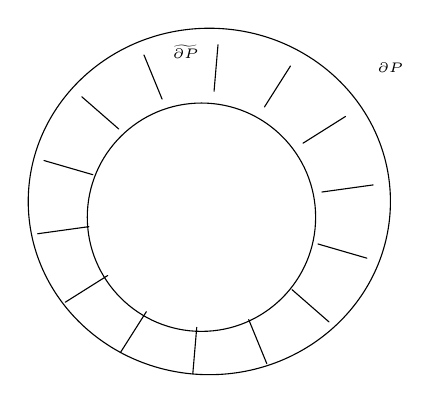
\begin{tikzpicture}[x=1mm,y=1mm,line cap=round,line join=round,font=\scriptsize]
\draw (70,-50) ellipse[x radius=23, y radius=22];
\draw (69,-52) ellipse[x radius=14.5, y radius=14.5];
\draw (83.8,-55.4) -- (90,-57.2);
\draw (80.5,-61.2) -- (85.2,-65.3);
\draw (75,-65) -- (77.3,-70.6);
\draw (68.4,-66) -- (67.9,-71.9);
\draw (62,-64) -- (58.7,-69.2);
\draw (57.1,-59.4) -- (51.7,-62.8);
\draw (54.7,-53.2) -- (48.2,-54.1);
\draw (55.2,-46.6) -- (49,-44.8);
\draw (58.5,-40.8) -- (53.8,-36.7);
\draw (64,-37) -- (61.7,-31.4);
\draw (70.6,-36) -- (71.1,-30.1);
\draw (77,-38) -- (80.3,-32.8);
\draw (81.9,-42.6) -- (87.3,-39.2);
\draw (84.3,-48.8) -- (90.8,-47.9);
\node[inner sep=1pt] at (67,-31) {\tiny $\widetilde{\partial P}$};
\node[inner sep=1pt] at (93,-33) {\tiny $\partial P$};
\end{tikzpicture}
\end{document}
